\section{Deadlock detection}
To enhance the solving speed of the sokoban solver, were a preprocessing scheme named deadlock detection applied on the map before the solver was applied to it, which enhanced the solving speed,  by minimizing the search space. \\

The scheme looks at the maps and finds possible deadlocks, and mark those positions, such that the solver knows that the diamond cannot be placed at those positions. \\

Deadlock position are positions, where the diamond can be pushed to, but not retrieved from. Position as such are corner,  or along the edges of two corners.  \\

%image
% Different Deadlock  situations
%	Corner
%	edge


The scheme starts by finding corners in the map. Corners are found by inspecting the neighboring map position. 
If current position is (i,j) and the element at that position is a '.', are the position before (i-1,j) above(i,j-1) and the diagonal (i-1,j-1) inspected to see if if (i,j ) could be a corner.  If it is a corner, it will be  marked with the letter 'D' and logged for further processing. \\

% image
%	 up-Left corner 
% 	 up-right corner
%  down-left corner
%  down-right corner

\begin{figure}[H]
    \centering
        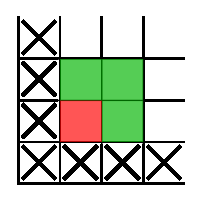
\includegraphics[width=0.40\textwidth]{images/deadlock_corner_leftup}
        \caption{One type of corner}
\end{figure}

When all the corners of the map is found, are these corners used to check whether the edge connecting these two corner also has to be deadlocked.   This is done by pairing the corners with corners that share the same row or column value, and then traverse one map position toward the other corner, while checking whether if the position contains a goal or diamond at which is shall not be deadlocked.\\

%
% Traversing edge

\begin{figure}[H]
    \centering
        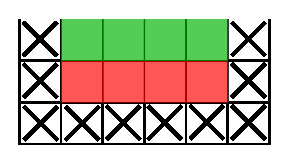
\includegraphics[width=0.40\textwidth]{images/deadlock_edge}
        \caption{Deadlocked edge between two corners}
\end{figure}


 At the same is its neighboring positions checked to make sure that the edge being traversed is end up becoming a wall which the diamond can't be pushed through. \\

 
 % Traversing edge
 %  dont create a wall
 \begin{figure}[H]
    \centering
        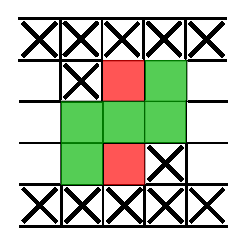
\includegraphics[width=0.40\textwidth]{images/deadlock_opposite}
        \caption{Traversing edge could create a wall here. }
\end{figure}
 
 
 Applying this scheme onto the map shows a great improvement of the solving speed,but also on the memory usage of the solver,  which the tests also shows. The low memory usage occurs as the amount of children declines, and thereby have a lower memory usage, and the search time declines as there is fewer children to search through. \\

\begin{figure}[H]
\centering
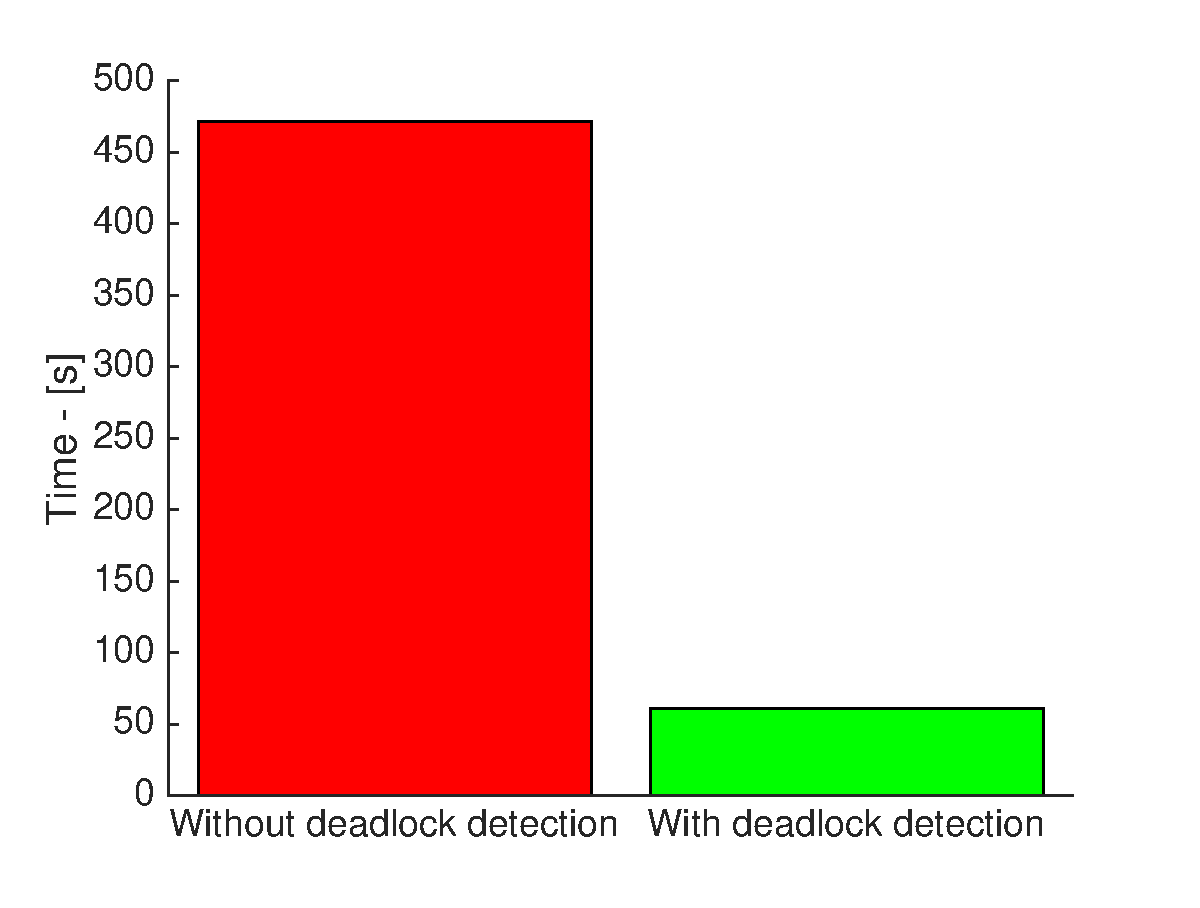
\includegraphics[width = \textwidth]{images/deadlockImprovement}
\caption{Improvement using deadlock detection}
\end{figure} 
 % Make test showing the memory usage with and without the solver 
 
 
An online version of an deadlock detection were also considered.  An online version could be capable while the system was solving the game, detect whether a child contained a deadlock state, and thereby remove it from the search.  This form of deadlocks could occur when a state has diamond located next to each other as such, such that each of them block each one. \\

 
% Online deadlock detection
% J J
% J J J 
% J J J J
% J J J J 
 
% J
% J

% J
% J
% J

% J
% J
% J
% J
 
This form deadlock detection would could also show a great enhancement in both solving speed, and memory usage. 
The problem with doing this form deadlock detection itself, is that new undefined deadlock cases would always occur,  and therefore making complete solution capable of  removing all the deadlock cases would be troublesome , at which it was decided to only perform it as a preprocessing scheme, and thereby remove the most obvious deadlocks, which has shown a great improvement in solving the game. 




